\documentclass[11pt,a4paper]{article}

\usepackage[utf8]{inputenc}
\usepackage[T1]{fontenc}
\usepackage[french]{babel}
\usepackage[a4paper,margin=2.4cm]{geometry}
\usepackage{graphicx}
\usepackage{booktabs}
\usepackage{array}
\usepackage{xcolor}
\usepackage{caption}
\usepackage{enumitem}
\usepackage{fancyhdr}
\usepackage{titlesec}
\usepackage[hidelinks]{hyperref}

\graphicspath{{figures/}}

\definecolor{nblue}{HTML}{1D3A6B}
\definecolor{acc}{HTML}{2563EB}
\definecolor{soft}{HTML}{EEF3FB}

\titleformat{\section}{\Large\bfseries\color{nblue}}{\thesection}{0.6em}{}
\titleformat{\subsection}{\large\bfseries\color{acc}}{\thesubsection}{0.6em}{}

\pagestyle{fancy}\fancyhf{}
\lhead{\small\color{nblue}AeroInsight AI — Analyse NLP des incidents ASRS}
\rhead{\small\thepage}
\renewcommand{\headrulewidth}{0.4pt}

\captionsetup{font=small,labelfont={bf,color=nblue}}
\newcommand{\kpi}[2]{\textbf{\color{acc}#1}\,\textemdash\,#2}

\begin{document}

% ---------------- TITLE ----------------
\begin{titlepage}
\centering
\vspace*{1.5cm}
{\small\color{acc}\textbf{AÉRONAUTIQUE \;|\; PROJET A3 \;|\; NLP · Classification · Clustering}}\\[1.2cm]
{\color{nblue}\Huge\bfseries Analyse NLP des rapports\\[0.3cm] d'incidents de sécurité aérienne\par}
\vspace{0.6cm}
{\large Extraction des causes récurrentes, classification des incidents\\ et détection de signaux faibles sur la base \textbf{NASA ASRS}\par}
\vspace{1.4cm}
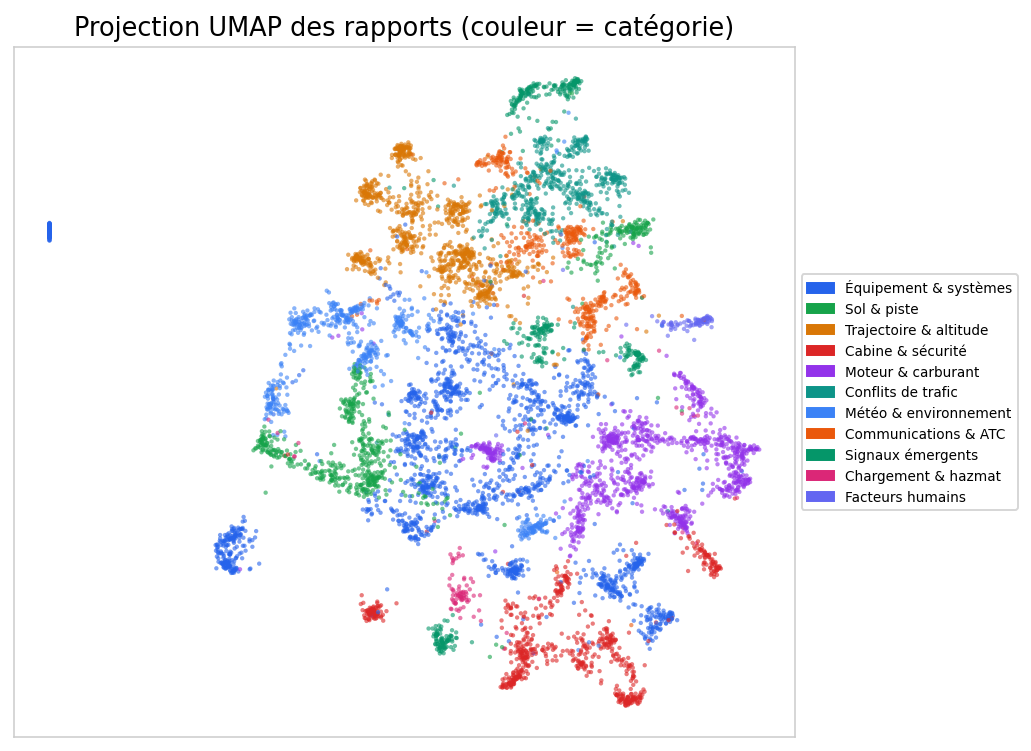
\includegraphics[width=0.92\textwidth]{scatter.png}\\[0.3cm]
{\small\itshape Projection sémantique des 125\,763 rapports — coloration par catégorie d'incident}
\vfill
\begin{tabular}{rl}
\textbf{Dataset} & NASA ASRS — 125\,763 rapports (2002–2025)\\
\textbf{Équipe} & 3 étudiants \;|\; 3–4 semaines\\
\textbf{Livrables} & Pipeline NLP · Dashboards (Streamlit \& React) · Rapport\\
\textbf{Dépôt} & \url{https://github.com/devMehdi485/asrs-ml}\\
\end{tabular}
\vspace{1cm}
\end{titlepage}

\tableofcontents
\newpage

% ---------------- 1 ----------------
\section{Contexte et problématique}
Chaque année, pilotes, contrôleurs et techniciens soumettent volontairement et de
manière confidentielle des milliers de rapports d'incidents à la NASA via
l'\emph{Aviation Safety Reporting System} (ASRS). Chaque rapport contient un
\textbf{récit en texte libre} décrivant l'événement, accompagné de métadonnées
codées par des experts. Cette base constitue une mine d'informations sur les
risques systémiques de l'aviation, mais elle reste \textbf{largement inexploitée}
faute d'outils capables d'analyser automatiquement des dizaines de milliers de
narratives.

\medskip
\noindent\textbf{Problématique.} Comment faire parler automatiquement ces récits
pour (i) extraire les \emph{causes récurrentes} d'incidents, (ii) \emph{classifier}
les types d'incidents et (iii) détecter des \emph{signaux faibles} précurseurs
d'accidents ?

% ---------------- 2 ----------------
\section{Objectifs}
\begin{itemize}[leftmargin=1.4em]
  \item Construire un \textbf{pipeline NLP complet} : prétraitement $\rightarrow$ vectorisation $\rightarrow$ clustering.
  \item Faire émerger des \textbf{thèmes d'incidents} cohérents et interprétables (non supervisé).
  \item \textbf{Classifier} le type d'anomalie à partir du texte (supervisé).
  \item Repérer des \textbf{signaux faibles} (rapports atypiques) et analyser l'\textbf{évolution temporelle}.
  \item Livrer un \textbf{dashboard interactif} de qualité professionnelle.
\end{itemize}

% ---------------- 3 ----------------
\section{Données}
\textbf{Source.} NASA ASRS — \url{asrs.arc.nasa.gov/search/database.html} (accès libre).
L'outil officiel limite chaque export à 10\,000 rapports ; nous avons travaillé sur
un export complet de \textbf{125\,763 rapports} (2002–2025) afin d'obtenir une
couverture statistique et temporelle robuste.

\smallskip
\noindent\textbf{Variables clés} (taux de remplissage mesuré sur le corpus) :
\begin{itemize}[leftmargin=1.4em,nosep]
  \item \emph{Narratives} Reporter 1 \& 2 et \emph{Synopsis} (texte libre) — 100\,\%.
  \item Type d'\textbf{anomalie} (cible supervisée) — 99,7\,\% ; \textbf{phase de vol} — 95,9\,\% ; \textbf{type d'aéronef} — 98,9\,\% ; \textbf{date} — 100\,\%.
  \item Conditions météo, détecteur, problème principal, facteurs contributifs — partiellement remplis.
\end{itemize}
\noindent\textbf{Particularité technique.} Les exports ASRS comportent une
\emph{double ligne d'en-tête} (catégorie + sous-champ), gérée automatiquement par
le module de chargement (aplatissement et repérage des colonnes par mots-clés).

% ---------------- 4 ----------------
\section{Méthodologie}

\subsection{Prétraitement NLP}
Nettoyage des artefacts de désidentification (\texttt{ZZZ}, tokens masqués),
mise en minuscules, tokenisation, suppression des \emph{stopwords} (anglais +
liste métier aéronautique), puis \textbf{lemmatisation} (NLTK). Deux versions du
texte sont produites : une version « naturelle » (pour les embeddings de phrases)
et une version « sac-de-mots » lemmatisée (pour TF-IDF et LDA).

\subsection{Vectorisation}
\begin{itemize}[leftmargin=1.4em,nosep]
  \item \textbf{TF-IDF} (uni + bigrammes) : représentation creuse et interprétable, base de la classification et de la labellisation des clusters.
  \item \textbf{Word embeddings (word2vec)} : un modèle \texttt{gensim} Word2Vec entraîné sur le corpus capture la sémantique lexicale du domaine (cf. tableau~\ref{tab:w2v}).
  \item \textbf{Embeddings de phrases} (\texttt{sentence-transformers}, \texttt{all-MiniLM-L6-v2}) : représentation contextuelle dense, utilisée pour le clustering. Ce choix constitue une \emph{amélioration} par rapport à word2vec/GloVe (le brief), les embeddings de phrases capturant le sens global d'un récit plutôt que des mots isolés.
\end{itemize}

\subsection{Clustering thématique}
Les embeddings sont réduits par \textbf{UMAP} puis regroupés. Deux algorithmes sont
comparés sur les \emph{mêmes} données (tableau~\ref{tab:clust}) :
\textbf{K-Means} (granularité fixée pour l'interprétabilité) et \textbf{HDBSCAN}
(densité, gère le bruit). Une règle de décision explicite sélectionne le modèle
final ; un garde-fou rejette tout HDBSCAN dégénéré (\textless 6 clusters).
La modélisation \textbf{LDA} (Latent Dirichlet Allocation) complète l'analyse par
une vue probabiliste des thèmes, évaluée par la \textbf{cohérence $c_v$}.

\subsection{Interprétation des thèmes}
Pour chaque cluster : extraction des termes saillants par \textbf{c-TF-IDF},
\textbf{labellisation} (nom métier + description rédigée), \textbf{synthèse} et
narratives représentatives. Les 81 thèmes ont été regroupés en \textbf{11 catégories}
métier (figure~\ref{fig:cat}).

\subsection{Classification supervisée}
Cible : l'anomalie principale (top-8 classes les plus fréquentes). Modèles :
\textbf{Régression logistique} et \textbf{SVM linéaire} sur TF-IDF
(tableau~\ref{tab:clf}).

\subsection{Signaux faibles et analyse temporelle}
Détection d'\textbf{Isolation Forest} sur les embeddings réduits (complétée par le
bruit HDBSCAN) pour isoler les rapports atypiques. L'analyse temporelle agrège les
volumes mensuels, détecte les pics (z-score) et suit la part de chaque thème dans
le temps.

% ---------------- 5 ----------------
\section{Résultats}

\subsection{Cartographie thématique}
Le clustering produit \textbf{81 thèmes} fins et interprétables, regroupés en
11 catégories. L'équipement et les systèmes dominent (43,8\,\% du corpus), suivis
des incidents au sol/piste (13,3\,\%) et des écarts de trajectoire/altitude (7,8\,\%).

\begin{figure}[h]\centering
  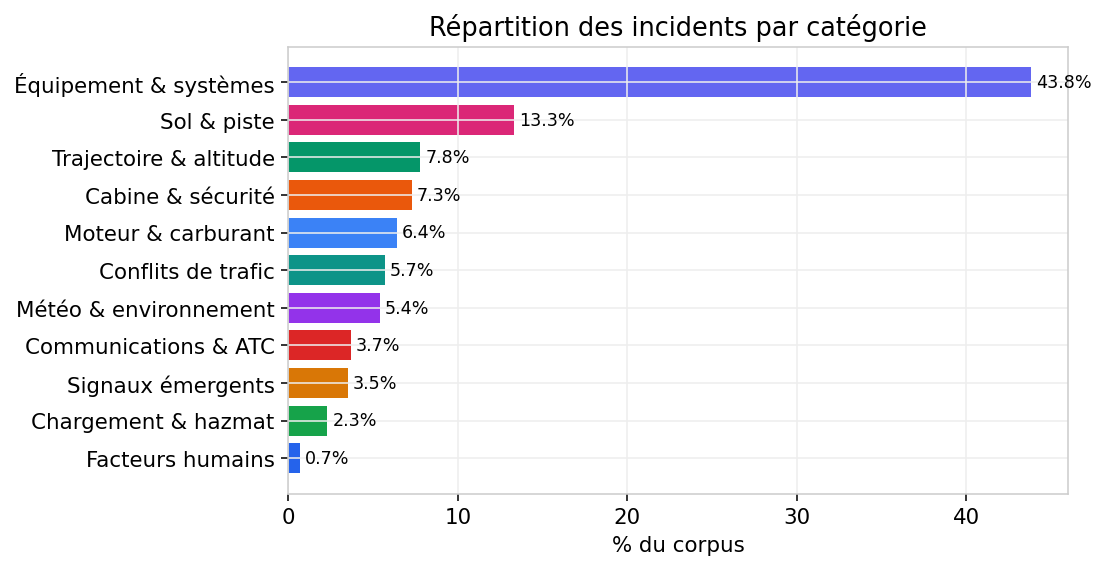
\includegraphics[width=0.86\textwidth]{categories.png}
  \caption{Répartition des incidents par catégorie métier.}\label{fig:cat}
\end{figure}

\begin{figure}[h]\centering
  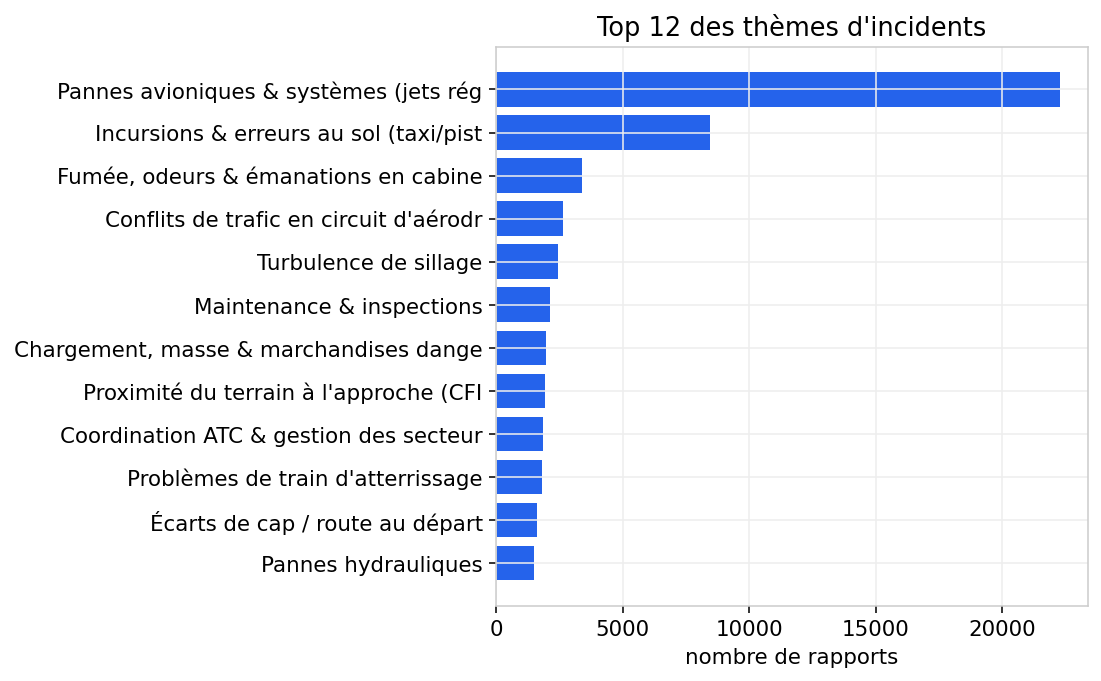
\includegraphics[width=0.86\textwidth]{top_themes.png}
  \caption{Principaux thèmes d'incidents (effectifs).}\label{fig:top}
\end{figure}

\begin{figure}[h]\centering
  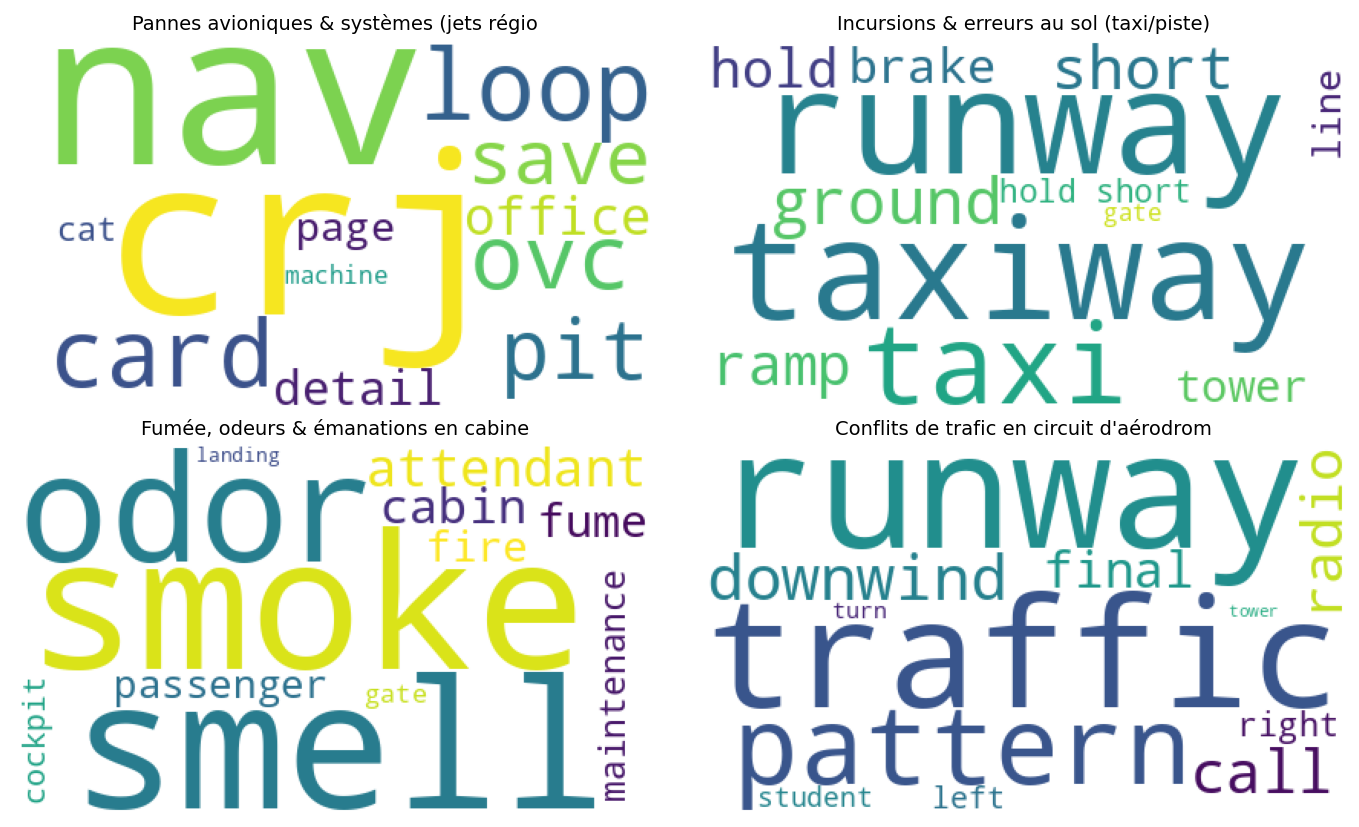
\includegraphics[width=0.95\textwidth]{wordclouds.png}
  \caption{Nuages de mots (c-TF-IDF) des quatre principaux thèmes.}\label{fig:wc}
\end{figure}

\subsection{Cohérence des clusters}
\begin{table}[h]\centering\small
\caption{Comparaison K-Means vs HDBSCAN (mêmes données réduites UMAP).}\label{tab:clust}
\begin{tabular}{lrrrrrr}
\toprule
\textbf{Modèle} & \textbf{Clusters} & \textbf{Silhouette} & \textbf{Davies-B.} & \textbf{Calinski-H.} & \textbf{Bruit} & \textbf{Pureté} \\
\midrule
K-Means  & 15 & 0,382 & 0,945 & 290\,094 & 0\,\% & 0,133 \\
\textbf{HDBSCAN} & \textbf{81} & \textbf{0,590} & \textbf{0,575} & 69\,804 & 32\,\% & 0,165 \\
\bottomrule
\end{tabular}
\end{table}
\noindent\textbf{Modèle retenu : HDBSCAN} — meilleure silhouette (0,590 vs 0,382) et
Davies-Bouldin plus faible, avec un taux de bruit (32\,\%) réutilisé pour la
détection de signaux faibles. La faible valeur d'ARI/pureté vis-à-vis du champ
\emph{Anomaly} est attendue : les thèmes sont sémantiques (vocabulaire des récits)
et plus fins que les catégories d'anomalies codées.

\subsection{Interprétabilité — modèle LDA \& word2vec}
La cohérence moyenne du modèle LDA atteint $c_v = 0{,}57$, signe de thèmes
lexicalement cohérents. Le modèle word2vec entraîné sur le corpus capture une
sémantique aéronautique fine :

\begin{table}[h]\centering\small
\caption{word2vec — mots les plus proches (similarité cosinus).}\label{tab:w2v}
\begin{tabular}{ll}
\toprule
\textbf{Mot} & \textbf{Voisins les plus proches} \\
\midrule
\texttt{runway}   & rwy (0,84), taxiway (0,65), intersecting (0,59), midfield (0,59) \\
\texttt{engine}   & eng (0,69), feathered (0,57), magneto (0,54), crossbleed (0,54) \\
\texttt{fuel}     & gas (0,69), gallon (0,60), fueled (0,60), gph (0,59) \\
\texttt{weather}  & thunderstorm (0,76), storm (0,74), bkn (0,68), forecast (0,66) \\
\texttt{altitude} & alt (0,70), descended (0,67), descend (0,65), level (0,64) \\
\texttt{gear}     & flap (0,62), slat (0,59), wheel (0,55), strut (0,52) \\
\bottomrule
\end{tabular}
\end{table}

\subsection{Classification supervisée}
\begin{table}[h]\centering\small
\caption{Classification du type d'incident (top-8 anomalies, TF-IDF).}\label{tab:clf}
\begin{tabular}{lrr}
\toprule
\textbf{Modèle} & \textbf{F1 macro} & \textbf{F1 pondéré} \\
\midrule
Régression logistique & 0,518 & 0,606 \\
SVM linéaire & 0,517 & \textbf{0,615} \\
\bottomrule
\end{tabular}
\end{table}
\noindent Les meilleures classes (\emph{ATC Issue} F1\,=\,0,76 ; \emph{NMAC} 0,69 ;
\emph{Aircraft Equipment Critical} 0,67) sont bien séparées ; les classes rares et
les anomalies multi-étiquettes restent plus difficiles.

\subsection{Évolution temporelle}
\begin{figure}[h]\centering
  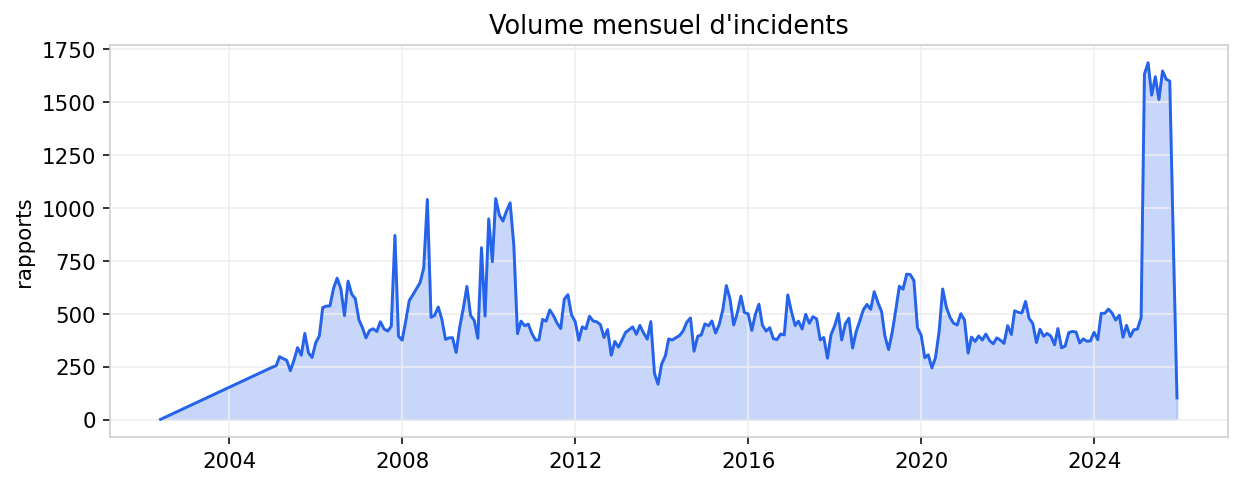
\includegraphics[width=0.9\textwidth]{temporal_volume.png}
  \caption{Volume mensuel de rapports (2002–2025).}\label{fig:vol}
\end{figure}
\begin{figure}[h]\centering
  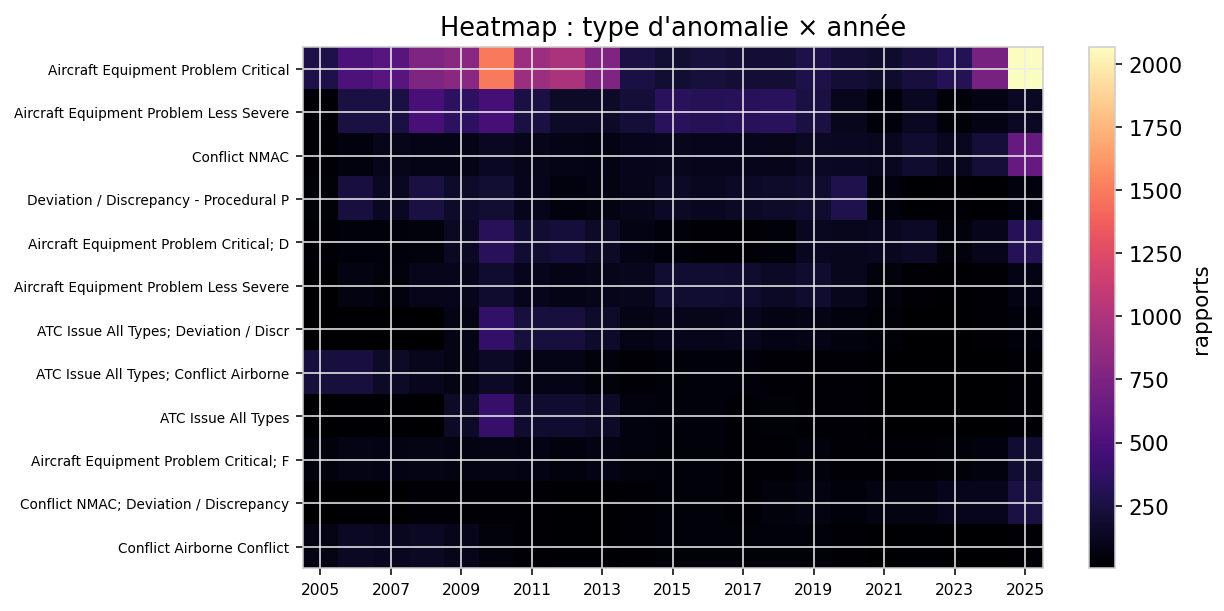
\includegraphics[width=0.9\textwidth]{heatmap.png}
  \caption{Heatmap : type d'anomalie × année.}\label{fig:heat}
\end{figure}
L'analyse des tendances révèle des thèmes en \textbf{hausse récente} —
incursions au sol, événements de fumée/odeur, drones, marchandises dangereuses —
candidats prioritaires pour un programme de sécurité.

\subsection{Causes récurrentes}
\begin{table}[h]\centering\small
\caption{Principales causes récurrentes (top 10).}\label{tab:causes}
\begin{tabular}{p{6.4cm}rrl}
\toprule
\textbf{Thème} & \textbf{Rapports} & \textbf{\%} & \textbf{Tendance} \\
\midrule
Pannes avioniques \& systèmes (jets régionaux) & 22\,258 & 26,2 & baisse \\
Incursions \& erreurs au sol (taxi/piste) & 8\,458 & 10,0 & hausse \\
Fumée, odeurs \& émanations en cabine & 3\,393 & 4,0 & hausse \\
Conflits de trafic en circuit d'aérodrome & 2\,657 & 3,1 & hausse \\
Turbulence de sillage & 2\,459 & 2,9 & stable \\
Maintenance \& inspections & 2\,108 & 2,5 & stable \\
Chargement, masse \& marchandises dangereuses & 1\,959 & 2,3 & hausse \\
Proximité du terrain à l'approche (CFIT) & 1\,906 & 2,2 & stable \\
Coordination ATC \& gestion des secteurs & 1\,858 & 2,2 & stable \\
Problèmes de train d'atterrissage & 1\,805 & 2,1 & stable \\
\bottomrule
\end{tabular}
\end{table}

% ---------------- 6 ----------------
\section{Dashboards}
Deux tableaux de bord ont été développés :
\begin{itemize}[leftmargin=1.4em,nosep]
  \item \textbf{Streamlit} (Python) — rapide à lancer, lit directement les artefacts.
  \item \textbf{AeroInsight AI} (React + TypeScript + Vite + Tailwind) — version web « pro »
  reproduisant la maquette, alimentée par un export JSON statique. Six pages :
  \emph{Dashboard, Cluster Explorer} (carte sémantique + filtres par catégorie),
  \emph{Thematic Analysis} (cartes de thèmes, LDA/pyLDAvis), \emph{Temporal Map},
  \emph{Weak Signals}, \emph{Executive Intelligence} (rapport auto-généré).
\end{itemize}
Chaque thème y est présenté avec un \textbf{nom métier lisible}, une description, des
\textbf{nuages de mots} et sa tendance temporelle.

% ---------------- 7 ----------------
\section{Adéquation aux critères d'évaluation}
\begin{table}[h]\centering\small
\renewcommand{\arraystretch}{1.25}
\begin{tabular}{p{3.4cm}p{10.5cm}}
\toprule
\textbf{Critère} & \textbf{Mise en œuvre} \\
\midrule
Cohérence des clusters & Comparaison K-Means/HDBSCAN (silhouette, Davies-Bouldin, Calinski-Harabasz), règle de décision justifiée, analyse qualitative. \\
Interprétabilité thématique & c-TF-IDF, labels métier + 11 catégories, LDA ($c_v=0{,}57$) + pyLDAvis, word2vec, tableau des causes. \\
Dimension temporelle & Volume mensuel, détection de pics, heatmap, topics-over-time. \\
Signaux faibles & Isolation Forest + bruit HDBSCAN. \\
Classification & Régression logistique \& SVM (F1 pondéré jusqu'à 0,615). \\
Qualité du dashboard & Deux dashboards, dont une app React 6 pages, nuages de mots par cluster et carte temporelle. \\
\bottomrule
\end{tabular}
\end{table}

% ---------------- 8 ----------------
\section{Limites et perspectives}
\textbf{Limites.} Texte désidentifié (perte d'information), déséquilibre des classes
d'anomalies, biais de déclaration volontaire, et un méga-cluster d'équipement
au vocabulaire technique hétérogène.
\textbf{Perspectives.} Embeddings de domaine aéronautique (fine-tuning),
classification multi-étiquettes, modélisation de séquences temporelles, et
BERTopic de bout en bout.

% ---------------- 9 ----------------
\section{Conclusion}
Le projet livre un pipeline NLP complet, validé sur \textbf{125\,763 rapports}
réels, produisant \textbf{81 thèmes interprétables} regroupés en 11 catégories,
une classification supervisée opérationnelle, une détection de signaux faibles et
deux dashboards interactifs. L'ensemble transforme une masse de récits bruts en une
\textbf{intelligence de sécurité} exploitable et lisible.

\vfill
\noindent\footnotesize\textit{Données : NASA Aviation Safety Reporting System
(\url{https://asrs.arc.nasa.gov/}). Code et dashboards :
\url{https://github.com/devMehdi485/asrs-ml}.}

\end{document}
